\chapter{Phương pháp tìm hiểu}
\label{Chapter3}

\noindent\textit{Chương này nhóm chúng em trình bày về những đóng góp của bài báo mà nhóm chúng em tìm hiểu được. Ở đây, nhóm chúng em tập trung vào việc xử lý vấn đề thiên lệch dữ liệu; bằng cách kết nối giữa bài toán xây dựng hệ thống gợi ý và suy luận nhân quả, nhóm em sử dụng phương pháp Inverse propensity scoring (IPS), một phương pháp thường được sử dụng trong suy diễn nhân quả, cho quá trình đánh giá và huấn luyện mô hình gợi ý. Sau đó, nhóm chúng em trình bày về hai phương pháp ước lượng propensity được trình bày ở phần trước là ``Naive Bayes'' và ``Logistic Regression''. Tiếp theo, nhóm em trình bày phương pháp ``Matrix factorization'' dựa trên propensity vừa tìm được. Sau cùng, nhóm em trình bày về các vấn đề của phương pháp IPS và một phương pháp khác có thể khắc phục được các vấn đề của IPS là ``Self Normalized Inverse Propensity Scoring'' (SNIPS).}

\section{Xem hệ thống gợi ý như một tác động điều trị}

Như đã trình bày ở ví dụ về thiên lệch dữ liệu, ta có thể thấy rằng việc người dùng đánh giá hoặc không đánh giá một sản phẩm có thể bị ảnh hưởng bởi rất nhiều yếu tố tiềm ẩn. Giống như việc khi ta muốn xem xét một loại thuốc hay một phương pháp điều trị nhất định có hiệu quả như thể nào đối với bệnh nhân, bất kể kết quả có tích cực hay tiêu cực thì cũng có thể bị ảnh hưởng bởi rất nhiều yếu tố tiềm ẩn. Cụ thể, giả sử ta tiến hành thử nghiệm phương pháp điều trị đó trên một nhóm bệnh nhân, sau đó ta theo dõi tình trạng bệnh của các bệnh nhân đó, và ta quan sát được sức khỏe của bệnh nhân có chuyển biến tích cực, liệu ta có thể kết luận được rằng phương pháp điều trị đó có thật sự hiệu quả không? Nếu xem xét kỹ lưỡng, có thể rằng phương pháp điều trị của ta có lẽ  khá đắt tiền nên chỉ những người có điều kiện kinh tế ổn định mới có xu hướng dễ tiếp xúc với phương pháp điều trị đó. Mà những người như vậy thì sẽ nhiều điều kiện thuận lợi để chăm sóc sức khỏe bản thân hơn, dẫn đến việc tình trạng bệnh của họ có chuyển biến tích cực hơn. Do đó việc kiểm tra được độ hiệu quả một phương pháp điều trị không hề đơn giản, người ta thường sử dụng các mô hình nhân quả. Nếu ta xem mỗi người dùng như một bệnh nhân, mỗi bộ phim ta gợi ý giống như một phương pháp điều trị hoặc một loại thuốc được thể hiện trong hình \ref{fig:3.0_treatment}, ta sẽ quan tâm đến việc người dùng có phù hợp với bộ phim mà ta gợi ý hay không, phim được gợi ý có khiến người dùng thích thú hay không. Từ đó ta có thể thấy bài toán gợi ý và bài toán được đưa ra khá tương đồng nhau, do đó ta cũng sử dụng ý tưởng giải quyết của các phương pháp nhân quả đối với bài toán xem xét hiệu quả điều trị để gợi ý sản phẩm.

\begin{figure}[h]
    \centering
    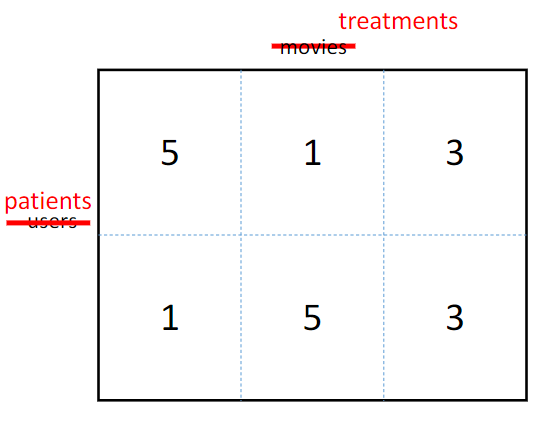
\includegraphics[width=\textwidth]{images/Chapter3/treatment.png}
    \caption{Mối liên hệ giữa hệ thống gợi ý và tác động điều trị.}
    \label{fig:3.0_treatment}
\end{figure}

Trong ví dụ về xem xét hiệu quả của một phương pháp điều trị, ta thấy được rằng ta không thể có được kết quả tình trạng bệnh của tất cả các bệnh nhân với tất cả các phương pháp điều trị như hình \ref{fig:3.0_treatment} mà chỉ có kết quả của các bệnh nhân tham gia điều trị hoặc tham gia thử nghiệm. Vậy nên, ta cần phải kiểm soát cả những biến làm ảnh hưởng đến khả năng bệnh nhân có thể tiếp cận được với điều trị đó để mô hình trở nên chính xác hơn, ví dụ như những đặc trưng về nhân khẩu học, thu nhập, mức sống, vị trí sống,... Tuy nhiên sẽ có rất nhiều biến ẩn như vậy mà ta khó có thể kiểm soát được. Do đó phương pháp Inverse propensity scoring (IPS) được nghiên cứu với ý tưởng rằng ta không cần phải kiểm soát trực tiếp những biến ẩn, mà chỉ cần kiểm soát được xu hướng nhận được điều trị của những bệnh nhân. Điều này vấn đúng với bài toán xây dựng hệ thống gợi ý, vì ta không thể kiếm biết được kết quả đánh giá của toàn bộ người dùng dành cho toàn bộ các bộ phim, cũng không thể kiểm soát những yếu tố tiềm ẩn, ví dụ như bộ phim đó có được gợi ý bởi bạn bè của người dùng hay không... Cho nên việc ta sử dụng một phương pháp phổ biến của suy diễn nhân quả cho bài toán xây dựng hệ thống gợi ý là hoàn toàn có cơ sở.

Trong bài toán gợi ý, với giả định rằng người dùng có thể đánh giá hoặc không đánh giá một phim mà họ đã xem, một đánh giá của người dùng dành cho một sản phẩm có thể xuất hiện hoặc không xuất hiện trong tập dữ liệu mà ta qua sát được. Ta có thể biểu diễn điều này thông qua ma trận quan sát O như trong hình \ref{fig:3.1_O}, trong đó các giá trị $O_{u,i}=1$ tương ứng với đánh giá cho bộ phim i từ người dùng u được cung cấp tới hệ thống. Ta đặt $P_{u,i}$ là xác suất mà đánh giá $Y_{u,i}$ được quan sát, hay  $P_{u,i} = P(O_{u,i} = 1)$.  $P_{u,i}$ được gọi là điểm propensity (propensity) của đánh giá  $Y_{u,i}$. Từ các đặc trưng mà ta đã quan sát được về các người dùng, các bộ phim và ma trận quan sát O, ta có thể dự đoán được propensity của ma trận đánh giá Y. Phương pháp này sẽ được giới thiệu ở phần tiếp theo của khóa luận này.


\begin{figure}[h]
    \centering
    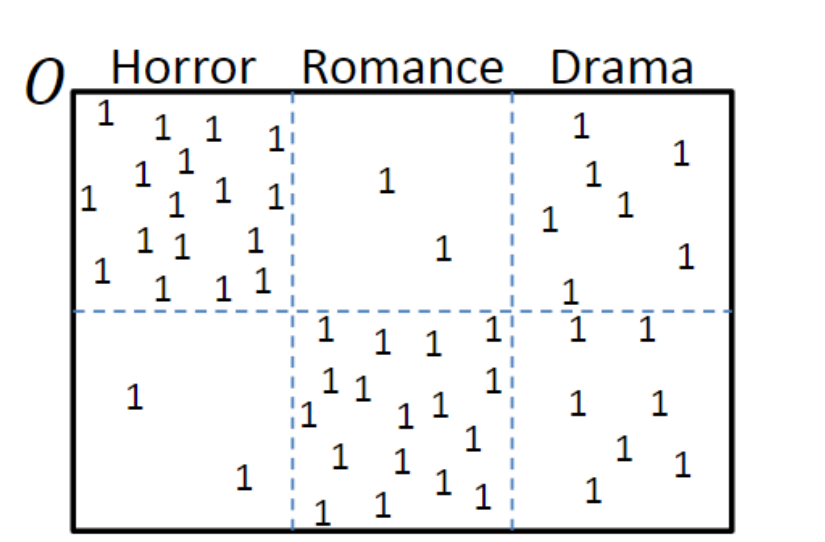
\includegraphics[width=\textwidth]{images/Chapter3/O.png}
    \caption{Hình ảnh minh họa ma trận quan sát O (hình ảnh được lấy từ bài báo của tác giả Tobias Schnabel \cite{IPS}).}
    \label{fig:3.1_O}
\end{figure}

\begin{figure}[h]
    \centering
    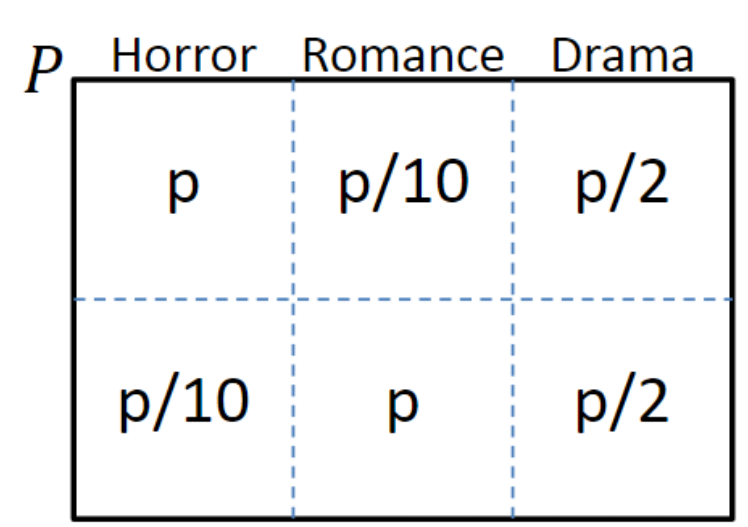
\includegraphics[width=\textwidth]{images/Chapter3/P.png}
    \caption{Hình ảnh minh họa ma trận quan sát P (hình ảnh được lấy từ bài báo của tác giả Tobias Schnabel \cite{IPS}).}
    \label{fig:3.1_P}
\end{figure}

Hình ảnh \ref{fig:3.1_P} và \ref{fig:3.1_O} minh họa về việc biểu diễn ma trận quan sát O và ma trận propensity P. Trong đó, ma trận quan sát O các vị trí có giá trị là 1 đại diện cho đánh giá của người dùng với sản phẩm xuất hiện trong hệ thống, ma trận propensity P chứa propensity của các đánh giá tương ứng với khả năng ta quan sát được các đánh giá, những phim có số lượt đánh giá nhiều sẽ có propensity cao.

\section{``Inverse propensity scoring'' (IPS)}
\subsection{Các hàm độ lỗi truyền thống}
Nhắc lại về phương pháp tính độ lỗi mà ta thường sử dụng, ta ký hiệu ma trận đánh giá mà ta quan sát được là Y, ma trận đánh giá mà ta dự đoán là $\hat{Y}$. Với Y là ma trận thưa chứa đánh giá của các người dùng cho các sản phẩm trong hệ thống, do người dùng không thể nào xem được tất cả sản phẩm, vì vậy đây là một ma trận thưa với rất nhiều đánh giá bị thiếu. Ma trận đánh giá mà ta dự đoán $\hat{Y}$ là ma trận đã được được điền đầy đủ các đánh giá bị thiếu từ mà trận $Y$; cụ thể, đây là ma trận chứa đánh giá của tất cả người dùng cho tất cả sản phẩm. Mục tiêu của phương pháp tính độ lỗi là xem xét liệu ma trận dự đoán $\hat{Y}$ có phải là ma trận $\hat{Y}$ khi đã được điền đầy đủ các giá trị thiếu hay không. Vì vậy hàm tính độ lỗi của ta sẽ tính toán độ lỗi dựa trên sự khác biệt về điểm đánh giá trên ma trận $\hat{Y}$ khi so sánh với các đánh giá trên ma trận $Y$. Thông thường, hàm tính độ lỗi sẽ được biểu diễn như sau:
\begin{equation}
\label{eq:tradition}
R(\hat{Y}) = \frac{1}{U\cdot I}  \sum_{u=1}^{U} \sum_{i=1}^{I} \delta_{u,i}(Y,\hat{Y})
\end{equation}

Trong đó, $\delta$ là một hàm tính độ lỗi bất kì.
Nhưng vì ta chỉ có thể quan sát được một phần của toàn bộ đánh giá, do đó ta chỉ tính trung bình độ lỗi của các đánh giá quan sát được, ta tạm gọi hàm lỗi này là hàm lỗi ngây thơ (Naive), hàm lỗi này có công thức như sau:
\begin{equation}
\label{eq:naive}
R_{Naive}(\hat{Y}) = \frac{1}{|\{(u,i):O_{u,i} = 1\}|} \sum_{(u,i):O_{u,i}=1}^{I} \delta_{u,i}(Y,\hat{Y}) 
\end{equation}


Sự ``ngây thơ'' của hàm lỗi này đã dẫn đến việc đánh giá mô hình bị sai ở ví dụ về thiên lệch lựa chọn trong phần \ref{section:thachthuc}. Do mẫu dữ liệu mà ta quan sát được không được phát sinh ngẫu nhiên theo phân phối đều từ dữ liệu thực tế mà bị thiên lệch, bắt nguồn từ việc người dùng tự lựa chọn các sản phẩm để đánh giá. Đó là lý do tại sao hàm lỗi ngây thơ lại có giá trị khác biệt so với độ lỗi thực tế, người ta gọi đây là một hàm lỗi bị lệch (bias), hay nói cách khác, kỳ vọng của hàm lỗi này khác với độ lỗi thực tế.
\[E_O [R_{Naive} (\hat{Y})] \ne R(\hat{Y})\]

\subsection{Hàm tính độ lỗi IPS}
Hiểu được vấn đề của hàm lỗi ngây thơ, nhóm tác giả đã đưa ra một hàm lỗi thay thế giúp giải quyết được vấn đề dữ liệu bị lệch. Phương pháp dựa trên một phương pháp thường được sử dụng trong các mô hình nhân quả, gọi là phương pháp Inverse propensity scoring (IPS). 

Áp dụng IPS trong nghiên cứu của Imbens và Rubin \cite{imbens_rubin_2015} để sử dụng cho hàm lỗi của hệ thống gợi ý, ta định nghĩa công thức tính độ lỗi IPS như sau:
\begin{equation}
\label{eq:IPS}
R_{IPS}(\hat{Y}|P) = \frac{1}{U\cdot I}\sum_{(u,i):O_{u,i}=1} \frac{\delta_{u,i}(Y,\hat{Y})}{P_{u,i}}
\end{equation}

Về cơ bản, propensity này luôn luôn lớn hơn 0 ở mọi cặp người dùng - sản phẩm để chắc chắn mỗi phần tử trong ma trận đánh giá Y đều có thể được quan sát; và tổng nghịch đảo các propensity của các đánh giá mà ta quan sát được sẽ bằng với số lượng đánh giá của toàn bộ người dùng dành cho toàn bộ sản phẩm, hay nói cách khác:

\begin{equation}
\label{eq:EO}
\mathbb{E}_{O}\bigg[\sum_{(u,i):O_{u,i}=1} \frac{1}{P_{u,i}}\bigg] = U \cdot I
\end{equation}

\begin{lemma}
(Sự không thiên lệch của IPS)
Với mọi người dùng u và sản phẩm i, nếu propensity $P_{u,i} \in (0,1)\text{ và }  P_{u,i}>0, \text{ thì }  R_{IPS}(\hat{Y}|P)$ là một độ đo không thiên lệch của $R(\hat{Y})$, có nghĩa là kỳ vọng của $R_{IPS}(\hat{Y}|P)$ bằng với $R(\hat{Y})$.
\end{lemma}

\textit{Chứng minh:} 
\begin{equation}
\begin{aligned}
\mathcal\mathbb{E}_{O} \Bigg[R_{IPS}(\hat{Y}|P)\Bigg] &=  \frac{1}{U\cdot I} \cdot \sum_{u=1}^{U} \sum_{i=1}^{I} \mathbb{E}_{O} \Bigg[ \frac{\delta_{u,i}(Y,\hat{Y}}{P_{u,i}}{O_{u,i}}\Bigg] \\ &= \frac{1}{U\cdot I} \cdot \sum_{u=1}^{U} \sum_{i=1}^{I}\delta_{u,i} \\ &
= R(\hat{Y})
\end{aligned}
\end{equation}

Trong phạm vi của bài báo mà nhóm em tìm hiểu, tác giả tiến hành hai loại nghiên cứu là nghiên cứu quan sát và nghiên cứu thực nghiệm:
\begin{itemize}
    \item Nghiên cứu thực nghiệm: trong nghiên cứu này, ta có thể điều khiển hệ thống gợi ý của ta bằng cách quyết định những sản phẩm nào sẽ được hiển thị đến người dùng, từ đó ta có thể biết được propensity của nó.
    \item Nghiên cứu quan sát: trong nghiên cứu này, ta không biết được propensity từ trước mà cần phải tiến hành ước lượng nó thông qua các thuộc tính của người dùng và sản phẩm; hoặc có thể thông qua dữ liệu đánh giá. Phương pháp ước lượng này sẽ được trình bài cụ thể trong phần tiếp theo thông qua các một trong hai mô hình ``Naive Bayes'' và ``Logistic Regression''.
\end{itemize}
\section{Ước lượng propensity}
\label{sec:3_estimate}
Trước tiên, để hiểu được các phương pháp ước lượng propensity của một đánh giá hay nói các khác là xác suất mà một đánh giá được quan sát, ta cần hiểu được các loại mất mát dữ liệu. Đầu tiêu là MAR (Mising At Random), có nghĩa là sự mất mát dữ liệu này là ngẫu nhiên. Kiểu mất mát này là kiểu ta thường giả định trong học máy. Ở kiểu mất mát này, ta có thể ước lượng được giá trị bị thiếu thông qua các giá trị quan sát được. Ví dụ như trong nghiên cứu về thông tin nhân khẩu học, nếu ta giả định rằng giá trị thu nhập bị thiếu là ngẫu nhiên thì ta có thể ước lượng thu nhập bị thiếu dựa vào các thông tin ta quan sát được như độ tuổi, nghề nghiệp, nơi sống,..Tuy nhiên,  một kiểu mất mát dữ liệu khác là MNAR (Missing Not At Random), ở kiểu mất mát này ta sẽ khó ước lượng được thu nhập bị thiếu vì các giá trị bị thiếu thường có một nguyên nhân nào đó, và nó mang một ý nghĩa nhất định.

Trong trường hợp trên, có thể những người dùng có thu nhập cao có xu hướng hạn chế công khai thu nhập của bản thân, do đó những thu nhập bị thiếu có thể cao hơn phần thu nhập ta quan sát được rất nhiều do đó không thể ước lượng bằng các mô hình học máy thông thường. Còn một kiểu mất mát khác là MCAR (Missing Completely At Random), có nghĩa là sự mất mát dữ liệu là hoàn toàn ngẫu nhiên, các mẫu mà ta quan sát được có thể xem như những mẫu đại diện, do đó ta có thể xóa những mẫu có dữ liệu bị thiếu. Ta có thể tìm hiểu kĩ hơn về các vấn đề mất mát dữ liệu trong nghiên cứu của \cite{rubin_2002}.

Xét nghiên cứu quan sát trên tập dữ liệu ML100K được cung cấp bởi Grouplens, ta dễ thấy các đánh giá bị thiếu không phải do ngẫu nhiên (MNAR) mà do thiên lệch lựa chọn của người dùng và của hệ thống gợi ý đã sử dụng. Do đó ta không biết được propensity của các đánh giá mà cần ước lượng propensity $P_{u,i}$ của mỗi đánh giá của người dùng u dành cho sản phẩm i sẽ được quan sát. Nói chung, xác suất một đánh giá ta có thể quan sát được có thể phụ thuộc vào các đặc trưng có thể quan sát được X (ví dụ như đặc trưng của người dùng, đặc trưng của sản phẩm mà ta thu thập được), các đặc trưng không thể quan sát được $X^{hid}$ (ví dụ như sản phẩm đó có được giới thiệu bởi bạn bè của người dùng hay không), và đánh giá Y:

\begin{equation}
\label{eq:pui}
    P_{u,i}=P(O_{u,i} = 1|X, X^{hid},Y)
\end{equation}

Do đó khi các đặc trưng có thể quan sát được đã được sử dụng để tính toán, ta có cơ sở để giả định rằng $O_{u,i}$ độc lập với ma trận dự đoán mới $\hat{Y}$ nên nó độc lập với $\delta_{u,i}(Y,\hat{Y})$.

Tiếp theo, ta làm rõ ý nghĩa của việc ước lượng ma trận propensity và hai phương pháp ước lượng ma trận propensity.

\begin{figure}[h]
    \centering
    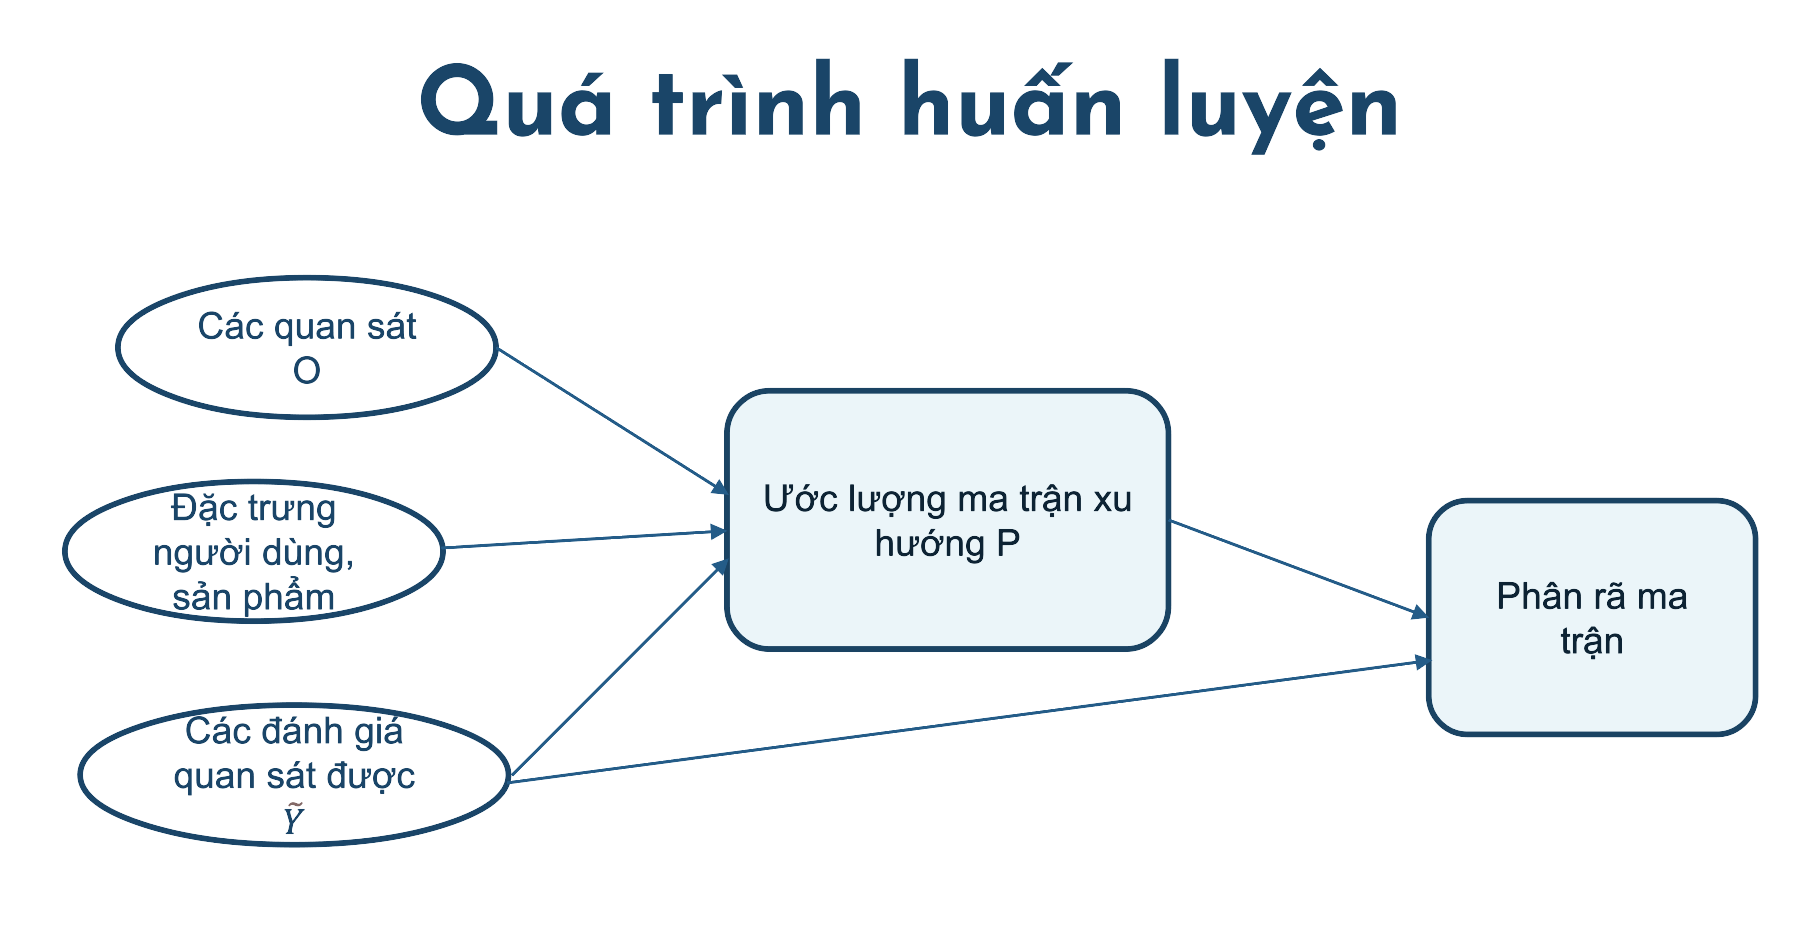
\includegraphics[width=\textwidth]{images/Chapter3/progress.png}
    \caption{Tóm tắt quá trình học.}
    \label{fig:3.3_progress}
\end{figure}

Hình \ref{fig:3.3_progress} cho thấy rằng ta sẽ sử dụng các thông tin về những đặc trưng có thể quan sát được X, ma trận quan sát O và ma trận đánh giá Y để ước lượng ma trận propensity. Cụ thể, phương pháp ``Naive Bayes'' sử dụng ma trận đánh giá Y và ma trận quán sát O, trong khi phương pháp ``Logistic Regression'' sử dụng các đặc trưng có thể quan sát X và ma trận quan sát O. Sau khi ước lượng ma trận propensity, ta sẽ sử dụng ma trận này kết hợp với ma trận đánh giá Y để sử dụng cho phương pháp MF-IPS sẽ được trình bày cụ thể trong \ref{sec:3_MFIPS}. 


\subsection{Ước lượng ma trận propensity thông qua ``Naive Bayes''}
\label{sec:3_estimate_NB}

Để thực hiện được phương pháp ``Naive Bayes'' cho ước lượng ma trận propensity, ta cần phải giả định rằng sự phụ thuộc giữa các biến X,   $X_{hid}$ và các đánh giá khác là không đáng kể. Do đó công thức \ref{eq:pui} được đơn giản thành $P(O_{u,i}|Y_{u,i})$ tương tự như nghiên cứu của nhóm tác giả Marlin và Zemel \cite{marlin2009}. Ta có thể xem $Y_{u,i}$ như là những mẫu đánh giá mà ta quan sát được, khi đó ta chỉ cần ước lượng các propensity cho những đánh giá quan sát được để tính toán IPS và SNIPS \cite{SNIPS}. Ta sử dụng mô hình ``Naive Bayes'' để ước lượng propensity này như sau:

\begin{equation}
\label{eq:pnb}
    P(O_{u,i} = 1| Y_{u,i} = r) = \frac{P(Y=r|O=1)P(O=1)}{P(Y=r)}
\end{equation}

Trong đó việc ước lượng maximum $P(Y=r|O=1)$ và $P(O=1)$ có thể được tính toán thông qua đếm số đánh giá  quan sát được trong dữ liệu MNAR. Tuy nhiên, khi muốn ước lượng $P(Y=r) = P(Y=r|O=1) + P(Y=r|O=0)$, ta cần phải có một mẫu nhỏ MCAR. Phương pháp cụ thể để tìm tập nhỏ MNAR sẽ được trình bày ở phần thực nghiệm.  

\subsection{Ước lượng ma trận propensity thông qua ``Logistic Regression''}
\label{sec:3_estimate_LR}
Một hướng tiếp cận khác để giải quyết việc  ước lượng ma trận propensity là sử dụng hồi quy Logistic. Phương pháp này có ưu điểm là không yêu cầu một tập mẫu nhỏ MCAR. Cũng dựa trên công thức \ref{eq:pui}, nhưng mục tiêu của ta là tìm một bộ tham số $\phi$ sao cho ma trận quan sát O có thể độc lập với ma trận ma
trận đặc trưng không quan sát được $X^{hid}$ và Y. Nói cách khác, $P(O_{u,i} = 1|X, X^{hid},Y) = P(O_{u,i}|X,\phi)$. Ở phương pháp này, ta giả định rằng tồn tại một bộ tham số $\phi=(\omega, \beta, \gamma)$ sao cho:

\begin{equation}
    \label{eq:plr}
    P_{u,i} = \sigma(\omega^TX_{u,i} + \beta_i + \gamma_u)
\end{equation}


Trong đó, $X_{u,i}$ là vector được vector hóa từ những thông tin quan sát được về các cặp người dùng, sản phẩm (ví dụ như thông tin nhân khẩu học của người dùng, bộ phim có được quảng cáo hay không), $\sigma(\cdot)$ là hàm sigmoid, $\beta_i, \gamma_u$ lần lượt là offset của người dùng và sản phẩm.


\section{``Matrix factorization'' kết hợp với IPS}
\label{sec:3_MFIPS}
Ở phần trước, ta đã tìm hiểu về phương pháp IPS ngoài ra ta còn tìm hiểu về cách ước lượng propensity của các đánh giá hay còn gọi là xác suất để các đánh giá xuất hiện trong tập dữ liệu mà ta quan sát được. Trong phần này, dựa vào những kiến thức đã trình bày trước đó, nhóm em sẽ sử dụng thay thế hàm lỗi của mô hình ``Matrix factorization'' bằng độ đo IPS dựa trên công thức \ref{eq:IPS}. 

Phát biểu bài toán: Với ma trận quan sát O, ma trận đánh giá Y, ma trận propensity P, không gian giả thuyết $\mathcal{H}$ của các dự đoán $\hat{Y}$ và hàm lỗi $\delta_{u,i}(Y, \hat{Y})$. Mục tiêu của ta là tìm $\hat{Y}$ sao cho:
\begin{equation}
    \label{eq:ERM}
    \hat{Y} = \underset{\hat{Y} \in \mathcal{H}}{argmin}\bigg\{\hat{R}_{IPS}(\hat{Y}|P\bigg\}
\end{equation}

Tiếp theo, để giải quyết bài toán dự đoán đánh giá $\hat{Y}$, ta sử dụng phương pháp ``Matrix factorization'' như đã trình bày ở chương \ref{section:MF}. Giả sử ta xem mô hình ``Matrix factorization'' với nhiệm vụ dự đoán mỗi đánh giá $\hat{Y}_{u,i} = \upsilon_u^T \omega_i + a_u + b_i + c$ với $a_u$ là  offset tương ứng của từng người dùng, $b_i$ là offset của sản phẩm, c là offset toàn cục của không gian giả thuyết $\mathcal{H}$. Từ đó ta có thể xem mục tiêu huấn luyện của ta là:

\begin{equation}
    \label{eq:objective}
    \underset{V,W,A}{argmin} \bigg[ \sum_{(u,i):O_{u,i}=1} \frac{\delta_{u,i}(Y,V^TW + A)}{P_{u,i}} + \lambda(||V||_{F}^2 + ||W||_{F}^2) \Bigg]
\end{equation}

Ta có thể thấy rằng, các phương pháp ``Matrix factorization'' truyền thống là một trường hợp đặc biệt của công thức \ref{eq:objective}, với tất cả propensity $P_{u,i}$ đều bằng nhau. Hay nói cách khác, khả năng xuất hiện của các đánh giá là như nhau, điều này xuất phát từ một giả định không chính xác của người dùng là dữ liệu đánh giá mà ta thu thập được là MCAR. Đây chính là điểm đặc biệt của mô hình mà nhóm em tìm hiểu. Mô hình này có vẻ không có quá nhiều khác biệt so với các mô hình thông thường được xây dựng trước đó, chỉ khác nhau một phần nhỏ ở hàm mục tiêu. Tuy nhiên, thách thức của việc tìm được ma trận propensity $P$ là khá lớn, và khó để tìm chính xác được một ma trận propensity $P$ để ta có thể thấy được toàn bộ dữ liệu thật sự dựa vào dữ liệu quan sát được. 

\section{``Self normalized inverse propensity scoring'' (SNIPS)}

Quay lại với nghiên cứu quan sát, khi mà ta chưa biết được giá trị của các propensity mà cần phải ước lượng chúng, việc ước lượng chính xác các propensity để tập dữ liệu ta quan sát được có thể đại diện cho toàn bộ tập tất cả dữ liệu gần như là một nhiệm vụ khó khăn. Tuy nhiên mục tiêu của ta không nhất thiết phải dự ước lượng một propensity hoàn hảo như vậy mà chỉ cần một propensity có tốt hơn so với việc xem tất cả các propensity là bằng nhau, tương tự như cách ta giả định rằng dữ liệu ta đang quan sát được là MCAR. Do đó, ma trận propensity mà ta ước lượng có thể có khác biệt lớn so với ma trận propensity hoàn hảo. Điều này dẫn đến việc ta cần xem xét một vài tính chất của ma trận propensity ước lượng được gây ảnh hưởng đến mô hình ``Matrix factorization''.

\begin{lemma}
Độ lệch của độ đo IPS với những propensity không chính xác: Đặt P là xác suất biên của việc quan sát được một đánh giá trong ma trận đánh giá Y, và đặt $\hat{P}$ là propensity được ước tính sao cho $\hat{P}_{u,i} > 0$ với mọi u,i. Độ lệch của độ đo IPS ở công thức \ref{eq:IPS} được tính theo công thức:

\begin{equation}
\label{eq:biasips}
bias\bigg (\hat{R}_{IPS}(\hat{Y}|\hat{P}) \bigg) = \sum_{u,i} \frac{\delta(Y, \hat{Y})}{U \cdot I} \Bigg[1-\frac{P_{u,i}}{\hat{P}_{u,i}}\Bigg]
\end{equation}
\end{lemma}

Ngoài vấn đề về độ lệch, ta còn cần phải quan tâm đến độ lỗi tổng quát của quá trình học, độ lỗi này bị ảnh hưởng như thế nào do tác động của propensity được ta ước lượng thông qua định lý được phát biểu trong \cite{IPS}, như sau:

\begin{theorem}[Giới hạn của độ lỗi tổng quát với phương pháp IPS]
    Với mọi không gian giả thuyết hữu hạn của các dự đoán $\mathcal{H} = \{\hat{Y}_1,...,\hat{Y}_{\mathcal{H}}\}$ và độ lỗi $0 \leqslant \delta_{u,i}(Y,\hat{Y}) \leqslant \Delta$, sử dụng độ đo IPS với ma trận propensity được ước lượng $\hat{P} (\hat{P}_{u,i} > 0)$ và cho ma trận quan sát O được huấn luyện từ Y với ma trận propensity P độc lập theo phân phối Bernoulli, được giới hạn bởi:
    
    \begin{equation}
    \begin{aligned}
        \label{eq:bound_erm}
        R(\hat{Y}) \leqslant \hat{R}_{IPS}(\hat{Y}|P) 
        & + \sum_{u,i} \frac{\delta(Y, \hat{Y})}{U \cdot I} \Bigg|1-\frac{P_{u,i}}{\hat{P}_{u,i}}\Bigg| \\ &+ \frac{\Delta}{U \cdot I} \sqrt{\frac{log(2|\mathcal{H}| / \eta}{2})} \sqrt{\sum_{u,i} \frac{1}{P^2_{u,i}}}
    \end{aligned}
    \end{equation}
    
\end{theorem}
Trong đó:
\begin{itemize}
    \item $\hat{R}_{IPS}(\hat{Y}|P)$ là độ lỗi IPS.
    \item $\sum_{u,i} \frac{\delta(Y, \hat{Y})}{U \cdot I} \Bigg|1-\frac{P_{u,i}}{\hat{P}_{u,i}}\Bigg|$ là độ lệch của độ lỗi IPS với ma trận propensity được ước lượng không hoàn hảo.
    \item $\frac{\Delta}{U \cdot I} \sqrt{\frac{log(2|\mathcal{H}| / \eta}{2})} \sqrt{\sum_{u,i} \frac{1}{P^2_{u,i}}}$ là phương sai của độ lỗi IPS với ma trận propensity được ước lượng không hoàn hảo.
\end{itemize}
Định lý trên cho thấy được sự đánh đổi giữa độ lệch và phương sai khác với các phương pháp học thông thường. Ở đây, ta có thể thấy rằng việc đánh giá cao những propensity nhỏ có thể có lợi nếu như việc giảm phương sai lớn hơn việc làm tăng độ lệch. Quay lại với công thức \ref{eq:IPS}, nếu ta thay thế propensity thực tế $P_{u,i}$ bằng propensity được ước lượng $\hat{P}_{u,i}$, ta được  $ \frac{1}{U \cdot I} \sum_{(u,i): O_{u,i} = 1} \frac{\delta_{u,i}(Y, \hat{Y}}{\hat{P}_{u,i}}$. Ở đây ta có thể thấy hai vấn đề có thể xảy ra với hàm lỗi IPS, đó là:
\begin{itemize}
    \item Ta đã biết rằng ta cố gắng ước lượng một ma trận propensity sao cho nó tốt hơn các propensity với phân phối đều, và có thể có sự khác nhau rất nhiều giữa các giá trị trong ma trận propensity. Nếu propensity của một đánh giá nào đó nhỏ hơn propensity của một đánh giá khác hàng trăm lần, thì độ lỗi của nó sẽ được khuếch đại lên gấp hàng trăm lần so với đánh giá khác.
    \item Ngoài ra, việc ta chỉ có thể ước lượng một ma trận propensity không hoàn hảo có thể khiến giá trị của propensity còn có nhiều khác biệt hơn.
\end{itemize}

Chính vì hai vấn đề trên, ta có thể thấy rằng độ lỗi IPS có thể biến thiên rất nhiều qua các lần huấn luyện, hay nói cách khác là độ lỗi IPS có phương sai lớn. Điều này khiến mô hình của chúng ta không được ổn định, đây là thứ ta phải đánh đổi cho một độ đo không thiên lệch. 

Để giải quyết vấn đề phương sai lớn của độ đo IPS, người ta đã áp dụng một kĩ thuật đó là sử dụng biến kiểm soát. Biến kiểm soát là một biến ngẫu nhiên mà ta biết được kỳ vọng của nó - là một công cụ được sử dụng để giảm phương sai của xấp xỉ Monte Carlo \cite{mcbook}. Đặt $V(X)$ là một biến kiểm soát với kỳ vọng được biết trước $\mathbb{E}_{X}[V(X)] = \upsilon \ne 0$ và đặt $\mathbb{E}_{X}[W(X)]$ là kỳ vọng mà ta muốn ước lượng dựa trên các mẫu độc lập của X. Ta có $\mathbb{E}_{X}[W(X)] = \frac{\mathbb{E}[W(X)]}{\mathbb{E}[V(X)]} \upsilon$. Từ đó ta có độ đo sau:

\begin{equation}
    \hat{W}^{SN} = \frac{\sum^n_{i=1} W (X_i)}{\sum^n_{i=1} V (X_i)} \upsilon
\end{equation}
 Độ đo trên được gọi là độ đo tự chuẩn hóa (Self-Normalized) trong các tài liệu về đánh lại trọng số của mẫu \cite{mcbook2}. Độ đo này được chứng minh rằng có phương sai giảm hơn đáng kể khi mà biến $W(X)$ và biến $V(X)$ có tương quan với nhau.
 
Dựa vào độ đo tự chuẩn hóa trên, nếu ta sử dụng $\sum_{(u,i):O_{u,i}=1} \frac{1}{P_{u,i}}$ như một biến kiểm soát cho độ đo IPS, ta biết được giá trị kỳ vọng của biến kiểm soát này theo công thức \ref{eq:EO} và ta dễ thấy biến ngẫu nhiên này có tương quan với độ đo IPS. Ta được độ đo SNIPS (Self-Normalized IPS) như sau: 

\begin{equation}
\begin{aligned}
    \label{eq:snips}
\hat{R}_{SNIPS}(\hat{Y}|P) &= \frac{\frac{1}{U \cdot I}\sum_{(u,i):O_{u,i}=1} \frac{ \delta_{u,i} (Y,\hat{Y}}{P_{u,i}})}{\sum_{(u,i):O_{u,i}=1} \frac{1}{P_{u,i}}} U \cdot I 
\\
\\ &= \frac{\sum_{(u,i):O_{u,i}=1} \frac{ \delta_{u,i} (Y,\hat{Y}}{P_{u,i}})}{\sum_{(u,i):O_{u,i}=1} \frac{1}{P_{u,i}}}
\end{aligned}
\end{equation}

Độ do SNIPS thường có phương sai nhỏ hơn IPS nhưng phải đánh đổi một chút độ lệch. 